% !TeX root = ../main.tex

\appendix{B}{Supplementary Scatter Plots for Cross-Cohort Feature Selection}

This appendix presents two-dimensional scatter plots of the most discriminative selected features under the \emph{cross-cohort} protocol (model trained on the 2020 cohort, projection and visualisation applied to the 2025 test cohort). These complement the within-cohort scatter plots shown in Figure~\ref{fig:fs_bilateral_scatter_comparison} of Chapter~\ref{chap:results}, and provide a visual characterisation of how well the selected feature subspace separates PD from healthy subjects when transferred to an unseen cohort recorded under a different protocol.

\section{Cross-Cohort Scatter Plots for Bilateral Feature Selection}

Figure~\ref{fig:fs_cross_scatter_comparison} shows the cross-cohort scatter plots for the three feature-selection methods applied to the bilateral hand-joint feature set (Experiment~2). Each plot projects the 2025 test subjects onto the two most discriminative features selected on the 2020 training cohort. PD subjects are shown in one colour and healthy subjects in another.

\begin{figure}[H]
  \centering
  \begin{subfigure}[t]{0.32\textwidth}
    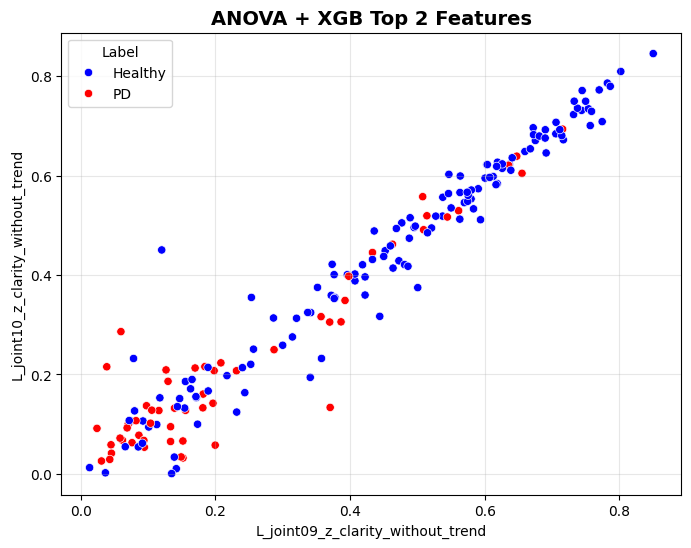
\includegraphics[width=\textwidth]{figures/cross_anova_fs_scatter.png}
    \caption{ANOVA, cross-cohort}
  \end{subfigure}
  \hfill
  \begin{subfigure}[t]{0.32\textwidth}
    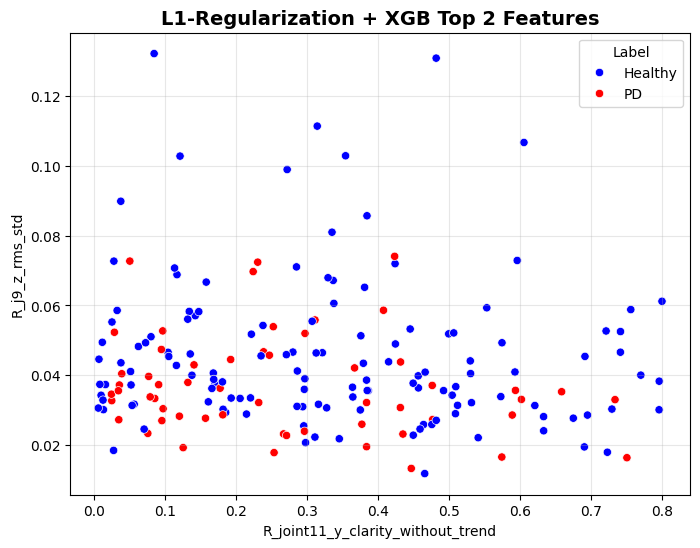
\includegraphics[width=\textwidth]{figures/cross_l1_fs_scatter.png}
    \caption{L1-Logistic, cross-cohort}
  \end{subfigure}
  \hfill
  \begin{subfigure}[t]{0.32\textwidth}
    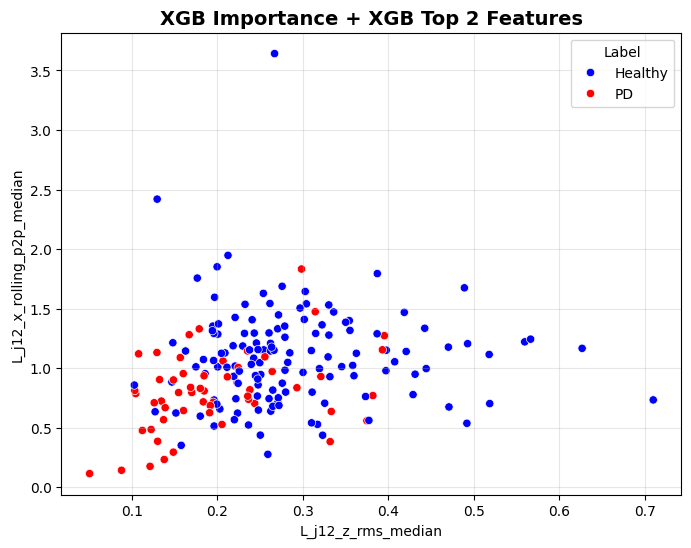
\includegraphics[width=\textwidth]{figures/cross_xgbimp_fs_scatter.png}
    \caption{XGB Importance, cross-cohort}
  \end{subfigure}
  \caption{Cross-cohort scatter plots of the two most discriminative selected features for each feature-selection method on bilateral hand-joint features (PD vs.\ healthy). Features are selected on the 2020 training cohort and applied to 2025 test subjects.}
  \label{fig:fs_cross_scatter_comparison}
\end{figure}

\section{Discussion}

Compared with the within-cohort scatter plots in Figure~\ref{fig:fs_bilateral_scatter_comparison}, the cross-cohort projections show reduced class separability. This visual degradation is consistent with the quantitative drop in AUROC reported in Table~\ref{tab:fs_bilateral_cross_dataset}: the feature dimensions most discriminative for the 2020 cohort do not retain the same discriminative geometry when projected onto the 2025 cohort. The overlap between PD and healthy clusters under all three selection methods corroborates the general finding that kinematic features selected on one recording protocol do not transfer perfectly to another, and provides a qualitative explanation for the ceiling on cross-cohort AUROC observed across Experiments~2--4.
